\documentclass[preprint,12pt]{elsarticle}

%% Use the option review to obtain double line spacing
%% \documentclass[preprint,review,12pt]{elsarticle}

%% Use the options 1p,twocolumn; 3p; 3p,twocolumn; 5p; or 5p,twocolumn
%% for a journal layout:
%% \documentclass[final,1p,times]{elsarticle}
%% \documentclass[final,1p,times,twocolumn]{elsarticle}
%% \documentclass[final,3p,times]{elsarticle}
%% \documentclass[final,3p,times,twocolumn]{elsarticle}
%% \documentclass[final,5p,times]{elsarticle}
%% \documentclass[final,5p,times,twocolumn]{elsarticle}

%% The graphicx package provides the includegraphics command.
\usepackage{graphicx}
%% The amssymb package provides various useful mathematical symbols
\usepackage{amssymb}
%% The amsthm package provides extended theorem environments
%% \usepackage{amsthm}

%% The lineno packages adds line numbers. Start line numbering with
%% \begin{linenumbers}, end it with \end{linenumbers}. Or switch it on
%% for the whole article with \linenumbers after \end{frontmatter}.
% \usepackage{lineno}

\usepackage{mathtools}
\usepackage{subcaption}

%% add pseudo codes
\usepackage{algorithm}
\usepackage{algorithmicx}
\usepackage{algpseudocode}

\floatname{algorithm}{Algorithm}
\renewcommand{\algorithmicrequire}{\textbf{INPUT:}}
\renewcommand{\algorithmicensure}{\textbf{OUTPUT:}}

%% add python codes
\usepackage{listings}
\usepackage{color}

\definecolor{dkgreen}{rgb}{0,0.6,0}
\definecolor{gray}{rgb}{0.5,0.5,0.5}
\definecolor{mauve}{rgb}{0.58,0,0.82}

\lstset{frame=tb,
  language=Python,
  aboveskip=3mm,
  belowskip=3mm,
  showstringspaces=false,
  columns=flexible,
  basicstyle={\small\ttfamily},
  numbers=none,
  numberstyle=\tiny\color{gray},
  keywordstyle=\color{blue},
  commentstyle=\color{dkgreen},
  stringstyle=\color{mauve},
  breaklines=true,
  breakatwhitespace=true,
  tabsize=3
}

%% natbib.sty is loaded by default. However, natbib options can be
%% provided with \biboptions{...} command. Following options are
%% valid:

%%   round  -  round parentheses are used (default)
%%   square -  square brackets are used   [option]
%%   curly  -  curly braces are used      {option}
%%   angle  -  angle brackets are used    <option>
%%   semicolon  -  multiple citations separated by semi-colon
%%   colon  - same as semicolon, an earlier confusion
%%   comma  -  separated by comma
%%   numbers-  selects numerical citations
%%   super  -  numerical citations as superscripts
%%   sort   -  sorts multiple citations according to order in ref. list
%%   sort&compress   -  like sort, but also compresses numerical citations
%%   compress - compresses without sorting
%%
%% \biboptions{comma,round}

% \biboptions{}

\journal{}

\begin{document}

\begin{frontmatter}

%% Title, authors and addresses

\title{Interpolation and Polynomial Approximation}

%% use the tnoteref command within \title for footnotes;
%% use the tnotetext command for the associated footnote;
%% use the fnref command within \author or \address for footnotes;
%% use the fntext command for the associated footnote;
%% use the corref command within \author for corresponding author footnotes;
%% use the cortext command for the associated footnote;
%% use the ead command for the email address,
%% and the form \ead[url] for the home page:
%%
%% \title{Title\tnoteref{label1}}
%% \tnotetext[label1]{}
%% \author{Name\corref{cor1}\fnref{label2}}
%% \ead{email address}
%% \ead[url]{home page}
%% \fntext[label2]{}
%% \cortext[cor1]{}
%% \address{Address\fnref{label3}}
%% \fntext[label3]{}


%% use optional labels to link authors explicitly to addresses:
%% \author[label1,label2]{<author name>}
%% \address[label1]{<address>}
%% \address[label2]{<address>}

\author{Xie Zhangqian}

\address{No.201600020098, Shandong University}

\begin{abstract}
%% Text of abstract
The purpose of this report is to approximate a function using polynomials and piecewise polynomials. Taken the accuracy and popularity into consideration, there are three methods discussed in the report, namely Newton's divided-difference formula, Hermite polynomial interpolation and cubic Hermite piecewise interpolation. Then several experiments have been made to verify the effectiveness of those interpolating methods. Based on results of those experiments, it can be observed that those methods are effective and useful to some extent. Though cubic Hermite piecewise interpolation has been introduced to approach Runge's phenomenon, the results are not very satisfied, in exact that the accuracy of approximation is asymmetric. Therefore, further discussions have been made to deal with the unsatisfied results, including using the cubic spline interpolation and generating more subintervals.
\end{abstract}

\begin{keyword}
Divided differences \sep Hermite interpolation \sep Piecewise-Polynomial approximation \sep Runge's Phenomenon
%% keywords here, in the form: keyword \sep keyword

%% MSC codes here, in the form: \MSC code \sep code
%% or \MSC[2008] code \sep code (2000 is the default)

\end{keyword}

\end{frontmatter}

%%
%% Start line numbering here if you want
%%
% \linenumbers

%% main text
\section{Introduction}
\label{S:1}

In the mathematical field of numerical analysis, interpolation is a method of constructing new data points within the range of a discrete set of known data points. In engineering and science, one often has a number of data points, obtained by sampling or experimentation, which represent the values of a function for a limited number of values of the independent variable. It is often required to interpolate, in exact, estimate the value of that function for an intermediate value of the independent variable.

A closely related problem is the approximation of a complicated function by a simple function. Suppose the formula for some given function is known, but too complicated to evaluate efficiently. A few data points from the original function can be interpolated to produce a simpler function which is still fairly close to the original. The resulting gain in simplicity may outweigh the loss from interpolation error.

Polynomials can be used to approximate complicated curves, for example, the shapes of letters in typography, given a few points. A relevant application is the evaluation of the natural logarithm and trigonometric functions: pick a few known data points, create a look-up table, and interpolate between those data points. This results in significantly faster computations. Polynomial interpolation also forms the basis for algorithms in numerical quadrature and numerical ordinary differential equations and Secure Multi Party Computation, Secret Sharing schemes.

Polynomial interpolation is also essential to perform sub-quadratic multiplication and squaring such as Karatsuba multiplication and Toom-Cook multiplication, where an interpolation through points on a polynomial which defines the product yields the product itself. In the case of Karatsuba multiplication this technique is substantially faster than quadratic multiplication, even for modest-sized inputs. This is especially true when implemented in parallel hardware.

A Newton polynomial, named after its inventor Isaac Newton, is an interpolation polynomial for a given set of data points. The Newton polynomial is sometimes called Newton's divided differences interpolation polynomial because the coefficients of the polynomial are calculated using Newton's divided differences method. Newton's formula is of interest because it is the straightforward and natural differences-version of Taylor's polynomial. Taylor's polynomial tells where a function will go, based on its $y$ value, and its derivatives (its rate of change, and the rate of change of its rate of change, etc.) at one particular $x$ value. Newton's formula is Taylor's polynomial based on finite differences instead of instantaneous rates of change.

Hermite interpolation, named after Charles Hermite, is a method of interpolating data points as a polynomial function. The generated Hermite interpolating polynomial is closely related to the Newton polynomial, in that both are derived from the calculation of divided differences.

Unlike Newton interpolation, Hermite interpolation matches an unknown function both in observed value, and the observed value of its first m derivatives. This means that $n(m+1)$ values must be known, rather than just the first $n$ values required for Newton interpolation. The resulting polynomial may have degree at most $n(m+1)-1$, whereas the Newton polynomial has maximum degree $n-1$. (In the general case, there is no need for $m$ to be a fixed value; that is, some points may have more known derivatives than others. In this case the resulting polynomial may have degree $N-1$, with $N$ the number of data points.)

In mathematics, a spline is a function defined piecewise by polynomials. In interpolating problems, spline interpolation is often preferred to polynomial interpolation because it yields similar results, even when using low degree polynomials, while avoiding Runge's phenomenon for higher degrees.

The term "spline" is used to refer to a wide class of functions that are used in applications requiring data interpolation and/or smoothing. The data may be either one-dimensional or multi-dimensional. Spline functions for interpolation are normally determined as the minimizers of suitable measures of roughness (for example integral squared curvature) subject to the interpolation constraints. Smoothing splines may be viewed as generalizations of interpolation splines where the functions are determined to minimize a weighted combination of the average squared approximation error over observed data and the roughness measure. For a number of meaningful definitions of the roughness measure, the spline functions are found to be finite dimensional in nature, which is the primary reason for their utility in computations and representation. For the rest of this section, we focus entirely on one-dimensional, polynomial splines and use the term "spline" in this restricted sense.

Before computers were used, numerical calculations were done by hand. Although piecewise-defined functions like the sign function or step function were used, polynomials were generally preferred because they were easier to work with. Through the advent of computers splines have gained importance. They were first used as a replacement for polynomials in interpolation, then as a tool to construct smooth and flexible shapes in computer graphics.

It is commonly accepted that the first mathematical reference to splines is the 1946 paper by Schoenberg, which is probably the first place that the word "spline" is used in connection with smooth, piecewise polynomial approximation. However, the ideas have their roots in the aircraft and shipbuilding industries. In the foreword to (Bartels et al., 1987), Robin Forrest describes "lofting", a technique used in the British aircraft industry during World War II to construct templates for airplanes by passing thin wooden strips (called "splines") through points laid out on the floor of a large design loft, a technique borrowed from ship-hull design. For years the practice of ship design had employed models to design in the small. The successful design was then plotted on graph paper and the key points of the plot were re-plotted on larger graph paper to full size. The thin wooden strips provided an interpolation of the key points into smooth curves. The strips would be held in place at discrete points (called "ducks" by Forrest; Schoenberg used "dogs" or "rats") and between these points would assume shapes of minimum strain energy. According to Forrest, one possible impetus for a mathematical model for this process was the potential loss of the critical design components for an entire aircraft should the loft be hit by an enemy bomb. This gave rise to "conic lofting", which used conic sections to model the position of the curve between the ducks. Conic lofting was replaced by what we would call splines in the early 1960s based on work by J. C. Ferguson at Boeing and (somewhat later) by M. A. Sabin at British Aircraft Corporation.

The use of splines for modeling automobile bodies seems to have several independent beginnings. Credit is claimed on behalf of de Casteljau at Citroën, Pierre B\'ezier at Renault, and Birkhoff, Garabedian, and de Boor at General Motors (see Birkhoff and de Boor, 1965), all for work occurring in the very early 1960s or late 1950s. At least one of de Casteljau's papers was published, but not widely, in 1959. De Boor's work at General Motors resulted in a number of papers being published in the early 1960s, including some of the fundamental work on B-splines.

Work was also being done at Pratt and Whitney Aircraft, where two of the authors of (Ahlberg et al., 1967)—the first book-length treatment of splines—were employed, and the David Taylor Model Basin, by Feodor Theilheimer. The work at General Motors is detailed nicely in (Birkhoff, 1990) and (Young, 1997). Davis (1997) summarizes some of this material.

Runge's phenomenon is a problem of oscillation at the edges of an interval that occurs when using polynomial interpolation with polynomials of high degree over a set of equispaced interpolation points. It was discovered by Carl David Tolm\'e Runge (1901) when exploring the behavior of errors when using polynomial interpolation to approximate certain functions. The discovery was important because it shows that going to higher degrees does not always improve accuracy. The phenomenon is similar to the Gibbs phenomenon in Fourier series approximations.

Section \ref{S:2} introduces concepts of three methods used to approximate a function with some given points. Those methods are Newton's divided-difference method, Hermite polynomial interpolation and cubic Hermite piecewise interpolation. Section \ref{S:3} illustrates several experiments to verify those methods respectively. Section \ref{S:4} makes some further discussions about the problems which has been encountered in previous experiments. Section \ref{S:5} gives an overview of full report.

\section{Methodologies}
\label{S:2}

There are several methods to approximate an unknown function with some given values, which have been introduced in \cite{burden:2001na}. In this section, three methods are to be illustrated, due to their popularity and accuracy. And there is a list of them below.

\begin{itemize}
\item Newton's divided-difference formula
\item Hermite polynomial interpolation
\item piecewise-polynomial interpolation
\end{itemize}

% \begin{enumerate}
% \item Numbered list item one
% \item Numbered list item two
% \end{enumerate}

All these methods can be used to approximate an unknown function with several different conditions. The Newton's divided-difference formula is a primitive approach to do approximation but not losing the accuracy in many cases. The Hermite polynomial interpolation is based on the concepts of osculating polynomials and some additional information of the function need to be given, in exact the first-order derivative values. The piecewise polynomial interpolation is a way to avoid some phenomena, such as Runge's phenomenon. And the piecewise polynomial can be realized with Hermite-type polynomials or splines interpolation.

\subsection{Newton's Divided-Difference Formula}
\label{SS:2.1}

Divided differences can be used to generate successively higher-degree polynomial approximations at a specific point, like the Lagrange interpolation mentioned in \cite{burden:2001na}. Such interpolation is sometimes called Newton interpolation. In fact, Lagrange interpolation is the same as the Newton interpolation, except for some difference in form. And the latter can be realized in program more easily so that only Newton interpolation is to be introduced in this report. The mathematical interpretation of divided-difference interpolation are followed.

Suppose that $P_{n}(x)$ is the $n$th Newton polynomial that agrees with the function $f$ at the distinct numbers $x_0,x_1,\dots,x_n$. The divided differences of $f$ with respect to $x_0,x_1,\dots,x_n$ are used to express $P_{n}(x)$ in the form

\begin{equation}
\label{eq:intro_dd1}
    P_{n}(x)=a_{0}+a_{1}(x-x_0)+a_{2}(x-x_0)(x-x_1)+\cdots+a_{n}(x-x_0)\cdots(x-x_{n-1}),
\end{equation}

for appropriate constants $a_0,a_1,\dots,a_n$. To determine the first of these constants, $a_0$, note that if $P_{n}(x)$ is written in the form of Eq. (\ref{eq:intro_dd1}), then evaluating $P_{n}(x)$ at $x_0$ leaves only the constant term $a_0$; that is, 

$$
a_0 = P_{n}(x_0)=f(x_0).
$$

Similarly, when $P_{n}(x)$ is evaluated at $x_1$, the only nonzero terms in the evaluation of $P_n(x_1)$ are the constant and linear terms, 

$$
f(x_0)+a_{1}(x_{1}-x_{0})=P_{n}(x_1)=f(x_1);
$$

so

\begin{equation}
\label{eq:intro_dd2}
    a_{1}=\frac{f(x_1)-f(x_0)}{x_{1}-x_{0}}.
\end{equation}

We now introduce the divided-difference notation, which is related to Aitken’s $\Delta^2$ notation. The \textit{zeroth divided difference} of the function $f$ with respect to $x_i$, denoted $f[x_i]$, is simply the value of $f$ at $x_i$: 

\begin{equation}
    f[x_i]=f(x_i).
\end{equation}

The remaining divided differences are defined recursively; the \textit{first divided difference} of $f$ with respect to $x_i$ and $x_{i+1}$ is denoted $f[x_i,x_{i+1}]$ and defined as 

\begin{equation}
    f[x_i,x_{i+1}]=\frac{f[x_{i+1}]-f[x_i]}{x_{i+1}-x_i}.
\end{equation}

The second divided difference, $f[x_i,x_{i+1},x_{i+2}]$, is defined as 

$$
f[x_i,x_{i+1},x_{i+2}]=\frac{f[x_{i+1},x_{i+2}]-f[x_{i},x_{i+1}]}{x_{i+2}-x_i}.
$$

Similarly, after the $(k-1)$st divided differences, 

$$
f[x_i,x_{i+1},x_{i+2},\dots,x_{i+k-1}]\quad \mathrm{and}\quad f[x_{i+1},x_{i+2},\dots,x_{i+k-1},x_{i+k}],
$$

have been determined, the \textbf{kth divided difference} relative to $$x_i,x_{i+1},x_{i+2}\dots,x_{i+k}$$
is 

\begin{equation}
    \begin{split}
        & f[x_{i},x_{i+1},\dots,x_{i+k-1},x_{i+k}]\\
        & =\frac{f[x_{i+1},x_{i+2},\dots,x_{i+k-1},x_{i+k}]-f[x_i,x_{i+1},x_{i+2},\dots,x_{i+k-1}]}{x_{i+k}-x_i}.
    \end{split}
\end{equation}

The process ends with the single \textit{$n$th divided difference},

$$
f[x_0,x_1,\dots,x_n]=\frac{f[x_1,x_2,\dots,x_n]-f[x_0,x_1,\dots,x_{n-1}]}{x_{n}-x_0}.
$$

Because of Eq. (\ref{eq:intro_dd2}) we can write $a_1 = f[x_0,x_1]$, just as $a_0$ can be expressed as $a_0 = f(x_0) = f[x_0]$. Hence the interpolating polynomial in Eq. (\ref{eq:intro_dd1}) is 

\begin{equation}
    \begin{split}
        P_{n}(x)= & f[x_0]+f[x_0,x_1](x-x_0)+a_{2}(x-x_0)(x-x_1)\\
        & +\cdots+a_{n}(x-x_0)(x-x_1)\cdots(x-x_{n-1}).
    \end{split}
\end{equation}

As might be expected from the evaluation of $a_0$ and $a_1$, the required constants are 

$$
a_k = f[x_0,x_1,x_2,\dots,x_k],
$$

for each $k=0,1,\dots,n$. So $P_{n}(x)$ can be rewritten in a form called Newton’s Divided Difference:

\begin{equation}
\label{eq:intro_dd3}
    P_{n}(x)=f[x_0]+\sum_{k=1}^{n} {f[x_0,x_1,\dots,x_k](x-x_0)\cdots(x-x_{k-1})}.
\end{equation}

The value of $f[x_0,x_1,\dots,x_k]$ is independent of the order of the numbers $x_0,x_1,\dots,x_k$, as shown in \cite{burden:2001na}.

\begin{algorithm}
    \caption{Newton's Divided-Difference Formula}
    \label{algo:dd}
    \begin{algorithmic}[1]
    \Require $\,x_0,x_1,\dots,x_n;\,f(x_0),f(x_1),\dots,f(x_n)\,\mathrm{as}\,F_{0,0},F_{1,0},\dots,F_{n,0}$.
    \Ensure the numbers $F_{0,0},F_{1,0},\dots,F_{n,0}$ where
    $$
    P_{n}(x)=F_{0,0}+\sum_{i=1}^{n}{F_{i,i}\prod_{j=0}^{i-1}{(x-x_j)}}.\quad (F_{i,i}\,is\,f[x_0,x_1,\dots,x_i].)
    $$
    \For{$i=1,2,\dots,n$}
        \For{$j=1,2,\dots,i$}
            \State $F_{i,j} \gets \frac{F_{i,j-1}-F_{i-1,j-1}}{x_{i}-x_{i-j}}.$ \Comment{($F_{i,j}=f[x_{i-j},\dots,x_i].$)}
        \EndFor
    \EndFor
    \State \textbf{OUTPUT} $(F_{0,0},F_{1,1},\dots,F_{n,n})$;
    \State \textbf{END}.
    \end{algorithmic}
\end{algorithm}

The pseudo codes of Newton's divided-difference formula are also shown in Algorithm \ref{algo:dd}.

\subsection{Hermite Polynomial Interpolation}
\label{SS:2.2}

\textit{Osculating polynomials} generalize both the Taylor polynomials and the Newton polynomials. Suppose that we are given $n+1$ distinct numbers $x_0,x_1,\dots,x_n$ in $[a,b]$ and non-negative integers $m_0,m_1,...,m_n$, and $m=max\{m_0,m_1,\dots,m_n\}$. The osculating polynomial approximating a function $f\in C^{m}[a,b]$ at $x_i$, for each $i=0,\dots,n$, is the polynomial of least degree that has the same values as the function $f$ and all its derivatives of order less than or equal to $m_i$ at each $x_i$. The degree of this osculating polynomial is at most

$$M=\sum_{i=0}^{n}{m_{i}}+n$$

because the number of conditions to be satisfied is $\sum_{i=0}^{n}{m_i}+(n+1)$, and a polynomial of degree $M$ has $M+1$ coefficients that can be used to satisfy these conditions.

The \textbf{osculating polynomial} approximating $f$ is the polynomial $P(x)$ of least degree such that 

$$\frac{d^{k}P(x_i)}{dx^{k}}=\frac{d^{k}f(x_i)}{dx^{k}},\quad\forall i=0,1,\dots,n;k=0,1,\dots,m_{i}.$$

Note that when $n = 0$, the osculating polynomial approximating $f$ is the $m_0$th Taylor polynomial for $f$ at $x_0$. When $m_i =0$ for each $i$, the osculating polynomial is the $n$th Lagrange polynomial interpolating $f$ on $x_0,x_1,\dots,x_n$.

The case when $m_i =1$, for each $i=0,1,\dots,n$, gives the Hermite polynomials. For a given function $f$, these polynomials agree with $f$ at $x_0,x_1,\dots,x_n$. In addition, since their first derivatives agree with those of $f$, they have the same “shape” as the function at $(x_i,f(x_i))$ in the sense that the \textit{tangent lines} to the polynomial and the function agree.

There is a method for generating Hermite approximations that has as its basis the Newton divided-difference formula (\ref{eq:intro_dd3}) at $x_0,x_1,\dots,x_n$. The alternative method uses the connection between the $n$th divided difference and the $n$th derivative of $f$.

Suppose that the distinct numbers $x_0,x_1,\dots,x_n$ are given together with the values of $f$ and $f^{'}$ at these numbers. Define a new sequence $z_0,z_1,\dots,z_{2n+1}$ by 

$$
z_{2i}=z_{2i+1}=x_i,\quad\forall i=0,1,\dots,n,
$$

and construct the divided difference that uses $z_0,z_1,\dots,z_{2n+1}$. 

Since $z_{2i}=z_{2i+1}=x_i$ for each $i$, we cannot define $f[z_{2i},z_{2i+1}]$ by the divided difference formula. However, the reasonable substitution in this situation is $f[z_{2i},z_{2i+1}]=f^{'}(z_{2i})=f^{'}(x_i)$, the entries below can be used:

$$f^{'}(x_0),f^{'}(x_1),\dots,f^{'}(x_n)$$

in place of the undefined first divided differences

$$f[z_0,z_1],f[z_2,z_3],\dots,f[z_{2n},z_{2n+1}].$$

The remaining divided differences are produced as usual, and the appropriate divided differences are employed in Newton’s divided-difference formula. Thus, the Hermite polynomial is then given by

$$H_{2n+1}(x)=f[z_0]+\sum_{k=1}^{2n+1}{f[z_0,\dots,z_k](x-z_0)\cdots(x-z_{k-1})}.$$

\begin{algorithm}
    \caption{Hermite Interpolation}
    \label{algo:hermite}
    \begin{algorithmic}[1]
    \Require $x_0,x_1,\dots,x_n;f(x_0),\dots,f(x_n);f^{'}(x_0),\dots,f^{'}(x_n).$
    \Ensure $Q_{0,0},Q_{1,1},\dots,Q_{2n+1,2n+1}\,\mathrm{where}$ \begin{equation}\nonumber
        \begin{split}
            H(x)=& Q_{0,0}+Q_{1,1}(x-x_0)+Q_{2,2}(x-x_0)^{2}+Q_{3,3}(x-x_0)^{2}(x-x_1)\\
            & Q_{4,4}(x-x_0)^{2}(x-x_1)^{2}+\cdots\\
            & Q_{2n+1,2n+1}(x-x_0)^{2}(x-x_1)^{2}\cdots(x-x_{n-1})^{2}(x-x_n).
        \end{split}
    \end{equation}
    \For{$i=0,1,\dots,n$}
        \State $z_{2i}\gets x_i;$
        \State $z_{2i+1}\gets x_i;$
        \State $Q_{2i,0}\gets f(x_i);$
        \State $Q_{2i+1,0}\gets f(x_i);$
        \State $Q_{2i+1,1}\gets f^{'}(x_i).$
        \If{$i\neq 0$}
            $$Q_{2i,1}\gets\frac{Q_{2i,0}-Q_{2i-1,0}}{z_{2i}-z_{2i-1}}.$$
        \EndIf
    \EndFor
    \For{$i=2,3,\dots,2n+1$}
        \For{$j=2,3,\dots,i$}
            \State $Q_{i,j}=\frac{Q_{i,j-1}-Q_{i-1,j-1}}{z_{i}-z_{i-j}}.$
        \EndFor
    \EndFor
    \State \textbf{OUTPUT} $(Q_{0,0},Q_{1,1},\dots,Q_{2n+1,2n+1});$
    \State \textbf{STOP}.
    \end{algorithmic}
\end{algorithm}

The pseudo codes of Hermite polynomial interpolation are illustrated in Algorithm \ref{algo:hermite}.

\subsection{Piecewise-Polynomial Interpolation}
\label{SS:2.3}

The previous sections concerned the approximation of arbitrary functions on closed intervals using a single polynomial. However, high-degree polynomials can oscillate erratically, that is, a minor fluctuation over a small portion of the interval can induce large fluctuations over the entire range. One example of that is \textbf{Runge's phenomenon}, which has been found by Runge on Runge function. Further discussions about it are in Section \ref{S:3.3}.

An alternative approach is to divide the approximation interval into a collection of subintervals and construct a (generally) different approximating polynomial on each subinterval. This is called \textbf{piecewise-polynomial approximation}.

The simplest piecewise-polynomial approximation is \textbf{piecewise-linear} interpolation, which consists of joining a set of data points 

$$\{(x_0,f(x_0)),(x_1,f(x_1)),\dots,(x_n,f(x_n))\}$$

by a series of straight lines, as shown in Figure \ref{fig:intro_pw1}.

\begin{figure}
\centering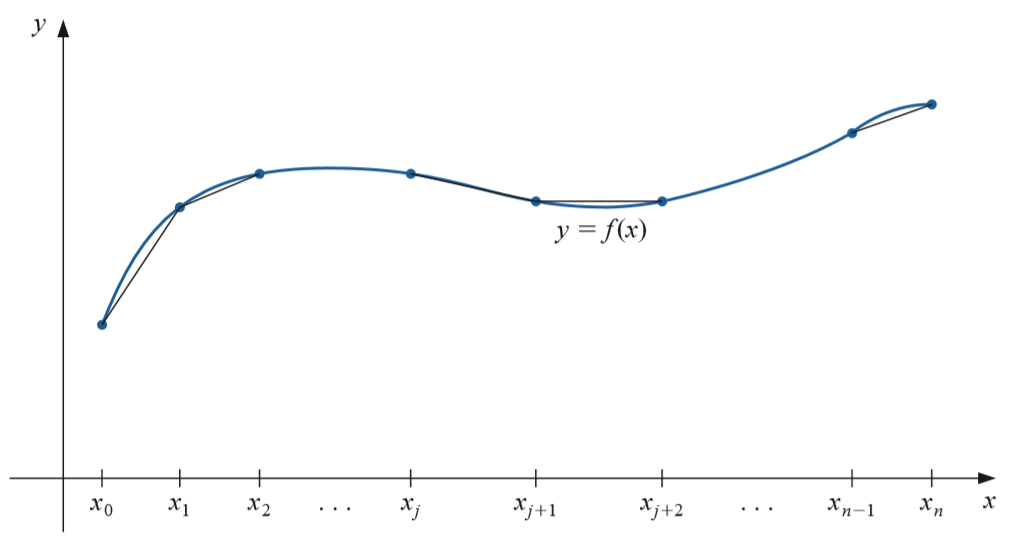
\includegraphics[width=0.4\linewidth]{piecewise_linear.png}
\caption{Piecewise-Linear interpolation}
\label{fig:intro_pw1}
\end{figure}

A disadvantage of linear function approximation is that there is likely no differentiability at the endpoints of the subintervals, which, in a geometrical context, means that the interpolating function is not “smooth.” Often it is clear from physical conditions that smoothness is required, so the approximating function must be continuously differentiable.

An alternative procedure is to use a piecewise polynomial of Hermite type. For example, if the values of $f$ and of $f^{'}$ are known at each of the points $x_{0}<x_{1}<\cdots<x_{n}$, a cubic Hermite polynomial can be used on each of the subintervals $[x_0,x_1],[x_1,x_2],\dots,[x_{n−1},x_n]$ to obtain a function that has a continuous derivative on the interval $[x_0,x_n]$.

To determine the appropriate Hermite cubic polynomial on a given interval is simply a matter of computing $H_3(x)$ for that interval. The Newton interpolating polynomials needed to determine $H_3$ are of first degree, so this can be accomplished without great difficulty. However, to use Hermite piecewise polynomials for general interpolation, we need to know the derivative of the function being approximated, and this is frequently unavailable.

\section{Experiments}
\label{S:3}

In this section, several experiments are made to verify efficiency and accuracy of three methods, which have been introduced in Section \ref{S:2}. To get the results of experiments, programs are written in Python and the following codes are run initially to import some useful packages and to set the style of plotting.

\begin{lstlisting}
import numpy as np
import matplotlib.pyplot as plt

plt.style.use('ggplot')
\end{lstlisting}

\subsection{Polynomial Interpolation of Divided Differences}

Given several known points which an unknown function passes through, the approximation of value of function at other points can be obtained by polynomial interpolation. As is mentioned in Section \ref{SS:2.1}, coefficients of polynomial interpolation can be achieved by divided differences so that the approximation can be done. To verify the effectiveness of divided-difference method, the function in Eq. (\ref{eq:dd1}) has been designed with four given values and $f(8.4)$ is to be approximated.

\begin{equation}
\label{eq:dd1}
\begin{split}
    f(8.1)=16.94410,\quad f(8.3)=17.56492,\\
    f(8.6)=18.50515,\quad f(8.7)=18.82091
\end{split}
\end{equation}

To approach this problem, define 

\begin{equation}
\label{eq:dd2}
    P_{n}(x)=a_{0}+a_{1}(x-x_0)+a_{2}(x-x_0)(x-x_1)+\cdots+a_{n}(x-x_0)\dots(x-x_{n-1})
\end{equation}

as a Newton polynomial to interpolate. Then input given points and do the iteration to get coefficients of Eq. (\ref{eq:dd2}). Running the program below, output the value of approximation, $f(8.4)=17.87714250$.

\begin{lstlisting}
## divided-differences
def newton_polynomial(x, initial_values, coefficients):
    
    poly = coefficients[0]
    for k in range(1, len(initial_values)):
        x_terms = 1
        for l in range(k):
            x_terms = x_terms * (x - initial_values[l])
        
        poly += coefficients[k] * x_terms
    
    return poly

x_inputs = [8.1, 8.3, 8.6, 8.7]
x_approx = 8.4

n = len(x_inputs)
F_array = np.zeros([n, n])

F_array[:, 0] = [16.94410, 17.56492, 18.50515, 18.82091]

for i in range(1, n):
    for j in range(1, i+1):
        F_array[i, j] = (F_array[i, j-1] - F_array[i-1, j-1]) / (x_inputs[i] - x_inputs[i-j])

print(F_array.round(5))
P_coeff = F_array.diagonal()
print('f({0})={1:.8f}'.format(x_approx, newton_polynomial(x_approx, x_inputs, P_coeff)))
\end{lstlisting}

The divided differences used in this problem are shown in Eq. (\ref{eq:dd3}), and coefficients of the Newton polynomial are on its main diagonal which have been underlined.

\begin{equation}
\label{eq:dd3}
    \begin{pmatrix}
        \underline{16.94410} & 0 & 0 & 0\\
        17.56492 & \underline{3.104100} & 0 & 0\\
        18.50515 & 3.134100 & \underline{0.060000} & 0\\
        18.82091 & 3.157600 &  0.058750 & \underline{-0.002080}
    \end{pmatrix}
\end{equation}

\subsection{Hermite Polynomial Interpolation}

Consider that more information about the unknown function has been given, like some derivative values, and indeed a more accurate approximation can be achieved through specific skills. As is mentioned in Section \ref{SS:2.2}, the Hermite polynomial, a kind of osculating polynomial, can be used to interpolate with introducing the derivative values. To verify the effectiveness of Hermite polynomials, a function is designed and the goal is to approximate $f(\frac{1}{3})$. The details of the function are shown in Table \ref{tab:hermite1}.

\begin{table}[h]
\centering
\begin{tabular}{l|l|l}
\textbf{$x_i$} & \textbf{$f(x_i)$} & \textbf{$f^{'}(x_i)$}\\
\hline
0.1 & −0.62049958 & 3.58502082 \\
0.2 & −0.28398668 & 3.14033271 \\
0.3 & 0.00660095 & 2.66668043 \\
0.4 & 0.24842440 & 2.16529366
\end{tabular}
\caption{The function to be approximated by Hermite polynomial}
\label{tab:hermite1}
\end{table}

To approach this problem, define 

\begin{equation}
\label{eq:hermite1}
    H_{2n+1}(x)=f[z_0]+\sum_{k=1}^{2n+1} {f[z_{0},\dots,z_{k}](x-z_0)(x-z_1)\cdots(x-z_{k-1})}
\end{equation}

as Hermite polynomial to interpolate, where

\begin{equation}
\label{eq:hermite2}
    z_{2i}=z_{2i+1}=x_i, \quad i=0,1,\dots,n.
\end{equation}

Then input given values and do the iteration to get coefficients of Eq. (\ref{eq:hermite1}). Running the program below, output the value of approximation, $f(\frac{1}{3})=0.09276343$.

\begin{lstlisting}
## Hermite
def newton_polynomial(x, initial_values, coefficients):
    
    poly = coefficients[0]
    for k in range(1, len(initial_values)):
        x_terms = 1
        for l in range(k):
            x_terms = x_terms * (x - initial_values[l])
        
        poly += coefficients[k] * x_terms
    
    return poly

x_inputs = [0.1, 0.2, 0.3, 0.4]
f_values = [-0.62049958, -0.28398668, 0.00660095, 0.24842440]
f_prime_values = [3.58502082, 3.14033271, 2.66668043, 2.16529366]
x_approx = 1/3

n = len(x_inputs)
F_array = np.zeros([2*n, 2*n])

z_values = []
temp_values = []
for m in range(n):
    z_values.extend([x_inputs[m], x_inputs[m]])
    temp_values.extend([f_values[m], f_values[m]])

F_array[:, 0] = temp_values
for i in range(n):
    F_array[2*i+1, 1] = f_prime_values[i]
    if i != 0:
        F_array[2*i, 1] = (F_array[2*i, 0] - F_array[2*i-1, 0]) / (z_values[2*i] - z_values[2*i-1])

for i in range(2, 2*n):
    for j in range(2, i+1):
        F_array[i, j] = (F_array[i, j-1] - F_array[i-1, j-1]) / (z_values[i] - z_values[i-j])

print(F_array.round(5))
P_coeff = F_array.diagonal()
print('f({0})={1:.8f}'.format(x_approx, newton_polynomial(x_approx, z_values, P_coeff)))    # set z_values as a hermite polynomial
\end{lstlisting}

The coefficients of Hermite polynomial are on the main diagonal of the matrix in Eq. (\ref{eq:hermite3}), which have been underlined.

\begin{equation}
\label{eq:hermite3}
    \begin{pmatrix}
        \begin{smallmatrix}
            \underline{-0.62050} & 0 & 0 & 0 & 0 & 0 & 0 & 0\\
            -0.62050 & \underline{3.58502} & 0 & 0 & 0 & 0 & 0 & 0\\
            -0.28399 & 3.36513 & \underline{-2.19892} & 0 & 0 & 0 & 0 & 0\\
            -0.28399 & 3.14033 & -2.24796 & \underline{-0.49045} & 0 & 0 & 0 & 0\\
            0.00660 & 2.90588 & -2.34456 & -0.48301 & \underline{0.03721} & 0 & 0 & 0\\
            0.00660 & 2.66668 & -2.39196 & -0.47395 & 0.04530 & \underline{0.04047} & 0 & 0\\
            0.24842 & 2.41823 & -2.48446 & -0.46250 & 0.05722 & 0.03972 & \underline{-0.00253} & 0\\
            0.24842 & 2.16529 & -2.52941 & -0.44949 & 0.06506 & 0.03923 & -0.00164 & \underline{0.00296}
        \end{smallmatrix}
    \end{pmatrix}
\end{equation}

\subsection{Piecewise Polynomial Interpolation of Hermite Type}
\label{S:3.3}

As is mentioned in Section \ref{SS:2.3}, high-degree polynomials can oscillate erratically, that is, a minor fluctuation over a small portion the interval can induce large fluctuations over the entire range. One example of such situation is called Runge's phenomenon due to Runge function which is shown in Eq. (\ref{eq:pw1}). Runge found that if this function is interpolated at equidistant points $x_i$ between $-1$ and $1$ with a polynomial $P_{n}(x)$ of degree $\leq n$, the resulting interpolation oscillates toward the end of the interval, in exact close to $-1$ and $1$. This shows that high-degree polynomial interpolation at equidistant points can be troublesome. (See Figure \ref{fig:pw1})

\begin{equation}
\label{eq:pw1}
    f(x)=\frac{1}{1+25x^2}, \quad x\in[-1,1]
\end{equation}

\begin{figure}[h]
\centering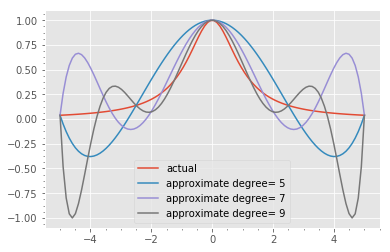
\includegraphics[width=0.4\linewidth]{Runge_phenomenon.png}
\caption{Runge phenomenon}
\label{fig:pw1}
\end{figure}

\begin{lstlisting}
## Runge Phenomenon
def newton_polynomial(x, initial_values, coefficients):
    
    poly = coefficients[0]
    for k in range(1, len(initial_values)):
        x_terms = 1
        for l in range(k):
            x_terms = x_terms * (x - initial_values[l])
        
        poly += coefficients[k] * x_terms
    
    return poly


def runge(x):
    return 1 / (1 + x ** 2)

xs = np.linspace(-5, 5, 100)
y = runge(xs)
plt.plot(xs, y, label='actual')

for deg in range(5, 11, 2):
    x_inputs = np.linspace(-5, 5, deg)
    f_values = runge(x_inputs)
    n = len(x_inputs)
    F_array = np.zeros([n, n])
    F_array[:, 0] = f_values
    for i in range(1, n):
        for j in range(1, i+1):
            F_array[i, j] = (F_array[i, j-1] - F_array[i-1, j-1]) / (x_inputs[i] - x_inputs[i-j])

    P_coeff = F_array.diagonal()
    ys = []
    for xss in xs:
        ys.append(newton_polynomial(xss, x_inputs, P_coeff))


    plt.plot(xs, ys, label='approximate degree= %d' % deg)

plt.legend()
plt.minorticks_on()
plt.show()
\end{lstlisting}

The problem can be avoided by using spline curves which are piecewise polynomials. When trying to decrease the interpolation error one can increase the number of polynomial pieces which are used to construct the spline instead of increasing the degree of the polynomials used. However, due to limited time, the following experiments just be based on the idea of piecewise polynomials and made through Hermite type rather than spline curves.

Firstly, do some transformation to simplify the derivative of Runge function. (See Eq. (\ref{eq:pw2}))

\begin{equation}
\label{eq:pw2}
    f(x)=\frac{1}{1+x^2}, \quad x\in[-5,5]
\end{equation}

Thus, the derivative of Eq. (\ref{eq:pw2}) is 

\begin{equation}
\label{eq:pw3}
    f^{'}(x)=\frac{-2x}{(1+x^2)^2}.
\end{equation}

Secondly, separate the interval into ten parts equidistantly. The goal is to approximate values of Eq. (\ref{eq:pw2}) at $-4,\,-3.5,\,-2,\,-1,\,0,\,1,\,2,\,3.5,\,4$. It is worth mentioned that the left part of Runge function can be approximated to a better accuracy, which is shown in Figure \ref{fig:pw2}. Such a flaw will be discussed in Section \ref{S:4}.

\begin{figure}[h]
\centering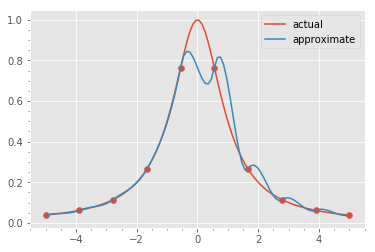
\includegraphics[width=0.4\linewidth]{runge_function.png}
\caption{Asymmetric approximation effect}
\label{fig:pw2}
\end{figure}

\begin{lstlisting}
## plot the forward-diff
xs = np.linspace(-5, 5, 100)
y = runge(xs)

ys = []
for xss in xs:
    if xss != xs[-1]:
        for sub_interval in input_interval:
            if sub_interval[0] <= xss < sub_interval[1]:
                sub_fval = runge(sub_interval)
                sub_fpval = runge(sub_interval)
                yss, _ = hermite_interpolation(xss, sub_interval, sub_fval, sub_fpval)
                ys.append(yss)
    else:
        ys.append(runge(xss))

plt.scatter(x_inputs, f_values)
plt.plot(xs, y, label='actual')
plt.plot(xs, ys, label='approximate')
plt.legend()
plt.minorticks_on()
plt.show()
\end{lstlisting}

Then input given values and do the iteration. Finally, run the program and the approximations have been obtained, which are shown in the Table \ref{tab:pw1}. And the details of interpolation error are illustrated in Table \ref{tab:pw2}.

\begin{lstlisting}
## piecewise Hermite
def newton_polynomial(x, initial_values, coefficients):
    
    poly = coefficients[0]
    for k in range(1, len(initial_values)):
        x_terms = 1
        for l in range(k):
            x_terms = x_terms * (x - initial_values[l])
        
        poly += coefficients[k] * x_terms
    
    return poly


def hermite_interpolation(x, initial_values, fval, fpval):
    
    n = len(initial_values)
    F_array = np.zeros([2*n, 2*n])

    z_values = []
    temp_values = []
    for m in range(n):
        z_values.extend([initial_values[m], initial_values[m]])
        temp_values.extend([fval[m], fval[m]])

    F_array[:, 0] = temp_values
    for i in range(n):
        F_array[2*i+1, 1] = fpval[i]
        if i != 0:
            F_array[2*i, 1] = (F_array[2*i, 0] - F_array[2*i-1, 0]) / (z_values[2*i] - z_values[2*i-1])

    for i in range(2, 2*n):
        for j in range(2, i+1):
            F_array[i, j] = (F_array[i, j-1] - F_array[i-1, j-1]) / (z_values[i] - z_values[i-j])

    P_coeff = F_array.diagonal()
    
    return newton_polynomial(x, z_values, P_coeff), P_coeff


def runge(x):
    return 1 / (1 + x ** 2)


def runge_derivative(x):
    return -2 * x / (1 + x ** 2) ** 2

x_inputs = np.linspace(-5, 5, 10)
f_values = runge(x_inputs)
f_prime_values = runge_derivative(x_inputs)
x_approxs = np.array([-4, -3.5, -2, -1, 0, 1, 2, 3.5, 4])

for x_approx in x_approxs:
    y_actual = runge(x_approx)
    y_direct, _ = hermite_interpolation(x_approx, x_inputs, f_values, f_prime_values)

    input_interval = []
    for l in range(len(x_inputs)-1):
        input_interval.append(x_inputs[l:l+2])

    for sub_interval in input_interval:
        if sub_interval[0] < x_approx < sub_interval[1]:    # make sure x_approx is not split point
            sub_fval = runge(sub_interval)
            sub_fpval = runge(sub_interval)
            y_piecewise, _ = hermite_interpolation(x_approx, sub_interval, sub_fval, sub_fpval)
    
    print('approximate f(%.1f)' % x_approx)
    print('actual: %.8f' % y_actual)
    print('direct: %.8f' % y_direct)
    print('piecewise: %.8f' % y_piecewise)
    print('direct absolute/relative:', round(abs(y_direct - y_actual), 5), round(abs(y_direct - y_actual) / y_actual, 5))
    print('piecewise absolute/relative:', round(abs(y_piecewise - y_actual), 5), round(abs(y_piecewise - y_actual) / y_actual, 5))
    print('-'*10)
\end{lstlisting}

As is depicted in Table \ref{tab:pw1}, the first column ("actual") means real values, the second column ("direct") means only using hermite interpolation on whole interval, and the third column ("piecewise") means results after adding piecewise polynomials.

\begin{table}[ht]
\centering
\begin{tabular}{l|l l l}
\textbf{approximate} & \textbf{actual} & \textbf{direct} & \textbf{piecewise}\\
\hline
$f(-4)$ & 0.05882353 & 0.02568213 & 0.05616445 \\
$f(-3.5)$ & 0.07547170 & -0.00617934 & 0.07691230 \\
$f(-2)$ & 0.20000000 & 0.19059916 & 0.19710715 \\
$f(-1)$ & 0.50000000 & 0.48800373 & 0.49431743 \\
$f(0)$ & 1.00000000 & 0.98082832 & 0.76415094 \\
$f(1)$ & 0.50000000 & 0.48800373 & 0.68237514 \\
$f(2)$ & 0.20000000 & 0.19059916 & 0.26751541 \\
$f(3.5)$ & 0.07547170 & -0.00617934 & 0.07683235 \\
$f(4)$ & 0.05882353 & 0.02568213 & 0.06655908
\end{tabular}
\caption{The results of piecewise-polynomial approximation}
\label{tab:pw1}
\end{table}

As is illustrated in Table \ref{tab:pw2}, the first column ("absolute") and the second column ("relative") mean respectively absolute error of and relative error of direct method. The third column ("absolute(pw)") and the fourth column ("relative(pw)") mean respectively absolute error of and relative error of piecewise-polynomial method. Compared the results of those columns, approximations of negative values are more accurate for piecewise-polynomial method than for direct method. But approximations of other values are not evidently better than direct method.

\begin{table}[htb]
\centering
\begin{tabular}{l|l l l l}
\textbf{approximate} & \textbf{absolute} & \textbf{relative} & \textbf{absolute(pw)} & \textbf{relative(pw)}\\
\hline
$f(-4)$ & 0.03314 & 0.5634 & 0.00266 & 0.0452 \\
$f(-3.5)$ & 0.08165 & 1.08188 & 0.00144 & 0.01909 \\
$f(-2)$ & 0.0094 & 0.047 & 0.00289 & 0.01446 \\
$f(-1)$ & 0.012 & 0.02399 & 0.00568 & 0.01137 \\
$f(0)$ & 0.01917 & 0.01917 & 0.23585 & 0.23585 \\
$f(1)$ & 0.012 & 0.02399 & 0.18238 & 0.36475 \\
$f(2)$ & 0.0094 & 0.047 & 0.06752 & 0.33758 \\
$f(3.5)$ & 0.08165 & 1.08188 & 0.00136 & 0.01803 \\
$f(4)$ & 0.03314 & 0.5634 & 0.00774 & 0.1315
\end{tabular}
\caption{The error of piecewise-polynomial approximation}
\label{tab:pw2}
\end{table}

Therefore, the introduction of piecewise polynomials certainly increase the accuracy of approximation to some extent. When it comes to negative $x$, piecewise method has taken an apparent advantage over the direct method (just use the interpolation on the whole interval). However, the results of piecewise method are sometimes worse than those of direct method.

\section{Further Discussion}
\label{S:4}

As is mentioned in Section \ref{S:3.3}, the piecewise-polynomial method just used by Hermite type can bring about asymmetric approximation effect, which is not robust. To approach this problem, some further trials have been made.

Firstly, the Newton backward–difference formula has been used to test whether the direction of approximation affect the results because the experiment in previous section is made by forward difference. However, such measure has never change the results which may indict that it is not due to the direction of difference. It is worth mentioned that the Stirling's formula is not tried due to the constraints of time.

Secondly, more subintervals have been added to test whether the number of subintervals can affect the results of approximation. Certainly, doubling number of subintervals from 10 to 20 increases the accuracy of approximation but the asymmetric approximation still occurs, which is shown in Figure \ref{fig:further1}.

\begin{figure}[h]
\centering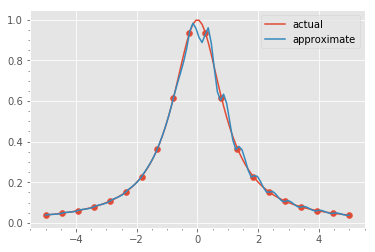
\includegraphics[width=0.4\linewidth]{runge_function_20.png}
\caption{Piecewise approximation with finer intervals separating}
\label{fig:further1}
\end{figure}

Finally, cubic spline interpolation have been used. The introduction of cubic spline interpolation certainly deal with the asymmetric approximation effect, which is depicted in Figure \ref{fig:further2}. The program is not written from the base and a ready-made package has been used due to limited time.

\begin{figure}[h]
\centering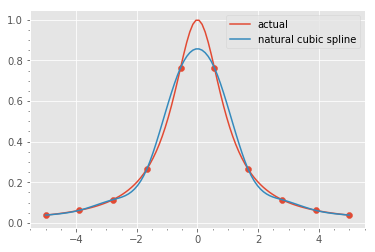
\includegraphics[width=0.4\linewidth]{cubic_spline.png}
\caption{Cubic spline interpolation}
\label{fig:further2}
\end{figure}

It deserves to be mentioned that natural cubic spline and clamped spline achieve the same results so only natural cubic spline has been illustrated in this report. Meanwhile, adding more subintervals also increases the accuracy of cubic spline interpolation.(See Figure \ref{fig:further3})

\begin{figure}[h]
\centering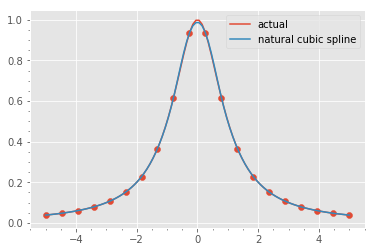
\includegraphics[width=0.4\linewidth]{cubic_spline_20.png}
\caption{Cubic spline interpolation with 20 subintervals}
\label{fig:further3}
\end{figure}

The programs used in this section are listed below.

\begin{lstlisting}
## cubic spline
from scipy.interpolate import CubicSpline

# x_inputs = np.linspace(-5, 5, 10)
x_inputs = np.linspace(-5, 5, 20)
f_values = runge(x_inputs)
f_prime_values = runge_derivative(x_inputs)

cs_natural = CubicSpline(x_inputs, f_values, bc_type='natural')
# cs_clamped = CubicSpline(x_inputs, f_values, bc_type=((1, f_prime_values[0]), (1, f_prime_values[-1])))

xs = np.linspace(-5, 5, 100)

ys_natural = cs_natural(xs)
ys_clamped = cs_natural(xs)

plt.scatter(x_inputs, f_values)
plt.plot(xs, runge(xs), label='actual')
plt.plot(xs, ys_natural, label='natural cubic spline')
# plt.plot(xs, ys_clamped, label='clamped cubic spline')
plt.legend()
plt.minorticks_on()
plt.show()
\end{lstlisting}

\section{Conclusion}
\label{S:5}

In this report, approximating a function using polynomials and piecewise polynomials have been considered. The function can be specified by a given defining equation or by providing points in the plane through which the graph of the function passes. A set of nodes $x_0,x_1,\dots,x_n$ is given in each case, and more information, such as the value of various derivatives, may also be required. We need to find an approximating function that satisfies the conditions specified by these data. The interpolating polynomial $P(x)$ is the polynomial of least degree that satisfies, for a function $f$,

$$P(x_i)=f(x_i),\quad\forall i=0,1,\dots,n.$$

Although this interpolating polynomial is unique, it can take many different forms. Newton’s forms of the polynomial are appropriate for computation and are also used extensively for deriving formulas for solving differential equations. However, polynomial interpolation has the inherent weaknesses of oscillation, particularly if the number of nodes is large. In this case there are other methods that can be better applied.

The Hermite polynomials interpolate a function and its derivative at the nodes. They can be very accurate but require more information about the function being approximated. When there are a large number of nodes, the Hermite polynomials also exhibit oscillation weaknesses.

The most commonly used form of interpolation is piecewise-polynomial interpolation. If function and derivative values are available, piecewise cubic Hermite interpolation is recommended. This is the preferred method for interpolating values of a function that is the solution to a differential equation. When only the function values are available, natural cubic spline interpolation can be used. This spline forces the second derivative of the spline to be zero at the endpoints. Other cubic splines require additional data. For example, the clamped cubic spline needs values of the derivative of the function at the endpoints of the interval.

After the introduction of those methods, several experiments have been made to verify the effectiveness and robustness of them. Based on results of the experiments, the statements in Section \ref{S:2} are mostly verified but there are still some disadvantage. Exactly, when it comes to research the Runge's phenomenon, an asymmetric approximation effect occurs, which indicts that more discussions are deserved. Thus, some discussion are made in Section \ref{S:4} and cubic spline interpolation is used in that section.

%% The Appendices part is started with the command \appendix;
%% appendix sections are then done as normal sections
% \appendix

% \section{}
% \label{}

%% References
%%
%% Following citation commands can be used in the body text:
%% Usage of \cite is as follows:
%%   \cite{key}          ==>>  [#]
%%   \cite[chap. 2]{key} ==>>  [#, chap. 2]
%%   \citet{key}         ==>>  Author [#]

%% References with bibTeX database:

\bibliographystyle{model1-num-names}
\bibliography{ref}

%% Authors are advised to submit their bibtex database files. They are
%% requested to list a bibtex style file in the manuscript if they do
%% not want to use model1-num-names.bst.

%% References without bibTeX database:

% \begin{thebibliography}{00}

%% \bibitem must have the following form:
%%   \bibitem{key}...
%%

% \bibitem{}

% \end{thebibliography}


\end{document}
